% --- To be compiled with XeLaTeX ---
% ---      Encoding: UTF-8        ---

\documentclass[a4paper, oneside, 11pt]{article}

%fontspec package provides a configurable interface for font selection, and allows complex font choices to be named and later reused. It's needed for XeLaTeX
\usepackage[cm-default]{fontspec}

% Unicode support
\usepackage{xunicode}
\usepackage{xltxtra}

% Default words and phrases in Greek (e.g. 'Περίληψη' instead of 'Abstract'). Also contains hyphenation rules for Greek Language
\usepackage{xgreek}

% Mathematical fonts, theorems etc.
\usepackage{amsfonts}
\usepackage{amsmath}
\usepackage{amsthm}

% Default page layout for consuming a larger portion of the page.
\usepackage{fullpage}

% Greek fonts (Computer Modern)
\setmainfont[Mapping=tex-text]{CMU Serif}

% Auxiliary commands
\newcommand{\red}{\leq_{\text{m}}}

\newtheorem{thm}{Θεώρημα}
\newtheorem{lm}[thm]{Λήμμα}

\theoremstyle{definition}
\newtheorem{defn}[thm]{Ορισμός}

\begin{document}

% Auxiliary commands
\newcommand{\HRule}{\rule{\linewidth}{0.5mm}}

\begin{titlepage}
\begin{center}


\includegraphics[width=0.3\textwidth]{../logos/pyrforos.png}
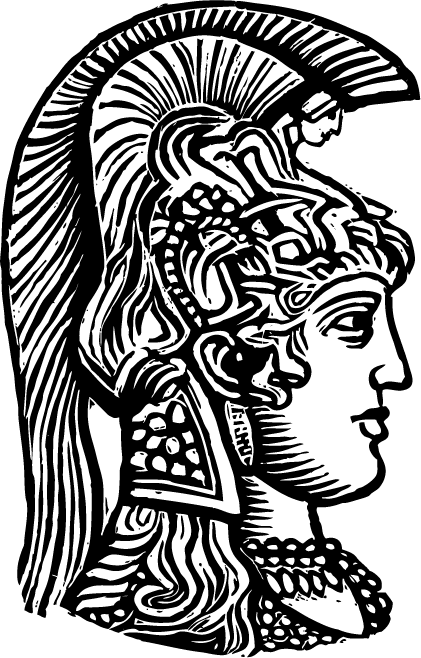
\includegraphics[width=0.2\textwidth]{../logos/uoa.png}\\[1cm]

\textsc{\LARGE Σχολή Ηλεκτρολόγων Μηχανικών και Μηχανικών Υπολογιστών}\\[1.5cm]

\HRule \\[0.4cm]
{\huge \bfseries Υπολογισιμότητα\\
\LARGE Ομάδα Ασκήσεων No. 2}\\[0.4cm]

\HRule \\[1.5cm]

\begin{center}
\textbf{Ομάδα}\\
Αξιώτης Κυριάκος\\
Αρσένης Γεράσιμος
\end{center}

\vfill

{\large \today}
\end{center}

\end{titlepage}


\section*{Άσκηση 1}
\section*{Άσκηση 2}
\section*{Άσκηση 3}
Έστω για κάθε $k\leq l$, 
$m_{k,l}(y)=\tau(k,\tau(k+1,\dots\tau(l,y)\dots))$. Θεωρούμε επίσης και την αντίστοιχη συνάρτηση $m(k,l,y)=m_{k,l}(y)$ για κάθε $k,l,y\in \mathbb{N}$ με $k\leq l$.

Τώρα, θεωρούμε για κάθε $x\in \mathbb{N}$ τις συναρτήσεις 

$n_{x+1}(y)=h(h(\dots h(h(g(m(0,x,y)),0,m(1,x,y)),1,m(2,x,y))\dots x-1,m(x,x,y)),x,y)$, και τώρα θεωρούμε
$f(0,y)=g(y)$ και $f(x+1,y)=n_{x+1}(y)$. Είναι εύκολο να επαληθεύσουμε ότι η $f$ ικανοποιεί τον αναδρομικό ορισμό της εκφώνησης. Συνεπώς είναι λύση αυτών των εξισώσεων.

Τώρα, για να δείξουμε ότι αν οι $g, h,\tau$ είναι Πρωτογενώς αναδρομικές, τότε είναι και η $f$, θα χρειαστεί να ορίσουμε κάποιες
συναρτήσεις.
Ορίζουμε

$a(0,k,y)=y$ και $a(c+1,k,y)=\tau(k-c-1,a(c,k,y))$

Η $a$ είναι εξ' ορισμού πρωτογενώς αναδρομική και εύκολα βλέπουμε ότι $a(c+1,k,y)=\tau(k-c-1,\tau(k-c,\dots\tau(k-1,y)\dots))$.

Ορίζουμε επίσης $b(x,k,y)=a(k-x-1,k,y)$. 

Τέλος, ορίζουμε

$f'(0,y,k)=g(a(k,k,y))$ και $f'(x+1,y,k)=h(f'(x,y,k),x,b(x,k,y))$. Προφανώς και η $f'$ είναι πρωτογενώς αναδρομική.

Εύκολα τώρα παρατηρούμε ότι $f(x,y)=f'(x,y,x)$, οπότε και η $f$ είναι πρωτογενώς αναδρομική.

\section*{Άσκηση 4}
\section*{Άσκηση 5}
\section*{Άσκηση 6}
Αν $p_1<p_2<...<p_n<...$ μία αρίθμηση των πρώτων αριθμών, ο αριθμός Goedel μιας ακολουθίας $x_1,x_2,...,x_n$ είναι ο
$x = p_1^{x_1}p_2^{x_2}\dots p_n^{x_n}$. το μήκος της ακολουθίας είναι το $n$.

(Θεωρούμε ότι οι λογικές τιμές T και F αντιστοιχούν στους ακεραίους $1$ και $0$ αντίστοιχα)
Ορίζουμε τη συνάρτηση $prime(i,x)$ η οποία επιστρέφει $1$ εάν ο $x$ δεν έχει διαιρέτη $\leq i+1$ και $0$ διαφορετικά.
Έχουμε $prime(i,x)=prime(i-1,x)\land x\ \mod\ (i+1)\neq 0$ και $prime(0,x)=1$, άρα η $prime$ είναι πρωτογενώς αναδρομική.
Επίσης θεωρούμε τη συνάρτηση $g(i,x)=prime(i)\land x\ \mod\ i=0$, η οποία ελέγχει εάν το $i$ είναι πρώτος παράγοντας του $x$ και
είναι πρωτογενώς αναδρομική. Τέλος, ορίζουμε $f(0,x)=0$ και $f(i+1,x)=g(i+1,x) + f(i,x)$, η οποία μετράει τους πρώτους παράγοντες
ενός αριθμού $x$ και είναι πρωτογενώς αναδρομική. Συνεπώς η συνάρτηση $F(x)=f(x,x)$ είναι πρωτογενώς αναδρομική και επιστρέφει
το μέγεθος της ακολουθίας που αντιστοιχεί στον αριθμό Goedel $x$.


\section*{Άσκηση 7}
Έστω $time(\langle M\rangle, x, t)$ η χρονικά περιορισμένη εκτέλεση της μηχανής $M$ με είσοδο $x$ σε χρόνο $t$. Αυτό σημαίνει ότι αν δεν τερματίσει σε χρόνο $t$, τότε απορρίπτει,
διαφορετικά έχει το αποτέλεσμα της $M(x)$.

a) Αρχικά, έχουμε ότι $L_{KENOTHTA}\in \Pi_1^0$, αφού το $\langle M\rangle\in L_{KENOTHTA}$ ισοδύναμα γράφεται ως $\forall x\forall t\ time(\langle M\rangle,x,t) rejects$. 
Αφού το κατηγόρημα είναι υπολογίσιμο, έχουμε ότι $L_{KENOTHTA}\in \Pi_1^0$.
Τώρα, θα δείξουμε ότι το συμπλήρωμα του προβλήματος τερματισμού (το οποίο είναι $\Pi_1^0$-πλήρες) ανάγεται στο $L_{KENOTHTA}$. Αυτό θα σημαίνει ότι και το τελευταίο είναι 
$\Pi_1^0$-πλήρες. Έστω μηχανή $M$ και είσοδος $x$ σε αυτήν. Κατασκευάζουμε μηχανή $M^{(x)}$ η οποία παίρνει είσοδο $y$. Την είσοδο την αγνοεί, και η λειτουργία της είναι
πανομοιότυπη με αυτήν της $M(x)$. Τώρα, αν η $M$ τερματίζει με είσοδο $x$, 
τότε και η $M^{(x)}(y)$ τερματίζει για όλα τα $y\in\Sigma^*$. Διαφορετικά, δεν τερματίζει για κανένα $y$.
Συνεπώς, η $M(x)$ δεν τερματίζει αν και μόνο αν $L(M^{(x)})=\emptyset$.

b) Αρχικά, έχουμε ότι $L_{\Pi\Lambda HPOTHTA}\in \Pi_2^0$, αφού το $\langle M\rangle\in L_{\Pi\Lambda HPOTHTA}$ ισοδύναμα γράφεται ως
$\forall x\exists t\ time(\langle M\rangle, x,t)\downarrow$. Προφανώς το κατηγόρημα είναι υπολογίσιμο, άρα αποδείχθηκε.
Τώρα, θα δείξουμε ότι οποιαδήποτε γλώσσα που περιγράφεται ως $\forall x\exists y\ \Phi (\mu, x,y)$ για κάποιο υπολογίσιμο κατηγόρημα $\Phi$ ανάγεται απεικονιστικά στο
$L_{\Pi\Lambda HPOTHTA}$.
Έστω μηχανή Turing $M$ η οποία παίρνει είσοδο $x$ και για όλα τα $y$ ελέγχει αν $\Phi(x,y)$. Αν βρει κάποιο τέτοιο $y$, τότε τερματίζει και επιστρέφει κάποια τιμή.
Διαφορετικά, δεν τερματίζει. Έχουμε ότι $\forall x\exists y\ Phi(x,y)$ αν και μόνο αν η $\phi_M$ είναι πλήρης.

c) Αρχικά, έχουμε ότι $L_{\Sigma YN\Pi E\Pi EPA\Sigma MENOTHTA}\in \Sigma_3^0$, αφού το $\langle M\rangle \in L_{\Sigma YN\Pi E\Pi EPA\Sigma MENOTHTA}$ ισοδύναμα γράφεται
ως $\exists n \exists (x_1, x_2, ..., x_n)\forall y\exists t (y\notin \{x_1, ..., x_n\} \rightarrow time(\langle M\rangle, y, t)\ accepts)$.

Για να δείξουμε τώρα ότι είναι πλήρες ως προς αυτήν την κλάση θα δείξουμε ότι κάθε γλώσσα $L\in \Sigma_3^0$ ανάγεται απεικονιστικά στην $L_{\Sigma YN\Pi E\Pi EPA\Sigma MENOTHTA}$.
Κατασκευάζουμε για δοθέν κατηγόρημα $\phi(x,y,z)$ τη μηχανή Turing $M$, η οποία παίρνει ως είσοδο ένα $y$ και ελέγχει παράλληλα για όλα τα $x$ αν 
$\forall y'\leq y\exists z\phi(x,y',z)$.
Αν κάποια στιγμή βρει κάποιο τέτοιο $x$, αποδέχεται. Διαφορετικά τρέχει για πάντα.

Αν $\exists x\forall y\exists z\ \phi(x,y,z)$, τότε η $M(y)$ αποδέχεται για όλα τα $y$. Συνεπώς $\overline{L(M)}=\emptyset$.


\section*{Άσκηση 8}
\section*{Άσκηση 9}
\section*{Άσκηση 10}
Έστω $K=\{\langle M\rangle\ |\ M(\langle M\rangle)\downarrow \}$ και ότι υπάρχει ιδιότητα $P\subseteq ER$ έτσι ώστε $L_P = K$. Έστω μηχανή Turing $Μ$ με είσοδο $x$
η οποία πρώτα υπολογίζει την κωδικοποίησή της και αν $x=\langle M\rangle$ η $M$ τρέχει για πάντα, ενώ διαφορετικά τερματίζει. Προφανώς $\langle M\rangle\notin K$.
Θεωρούμε τώρα μηχανή $M'$ ισοδύναμη με την $M$, αλλά με διαφορετική κωδικοποίηση, οπότε έχουμε $L(M')=L(M)$ και $\langle M'\rangle \in K$. 
Άρα $L(M)=L(M')\in P$ και $\langle M\rangle \in K$. 
Αυτό είναι
άτοπο αφού $\langle M\rangle\notin K$. Άρα το ζητούμενο αποδείχθηκε.

\section*{Άσκηση 11}
Γνωρίζουμε ότι οι γραμματικές τύπου $0$ είναι αυτές που αναγνωρίζονται απο μηχανές Turing σε πεπερασμένο χρόνο. Συνεπώς δοθείσας μιας γραμματικής $G$ υπάρχει μηχανή Turing
$M$ η οποία γράφει στην ταινία της διαδοχικά όλα τα στοιχεία της $L(G)$. Θα δείξουμε ότι η λειτουργία αυτής της μηχανής Turing μπορεί να προσομοιωθεί από μία γραμματική
με τους κανόνες της εκφώνησης. Μπορούμε επίσης να θεωρήσουμε ότι η $M$ κάθε φορά που βρίσκει μια λέξη τυπώνει τον ειδικό χαρακτήρα $\#$ που δεν εμφανίζεται πουθενά αλλού στη
μηχανή, τον οποίον στη συνέχεια αφαιρεί για να
συνεχίσει με τις υπόλοιπες λέξεις. Επίσης εισάγουμε έναν επιπλέον ειδικό χαρακτήρα $*$. 
Θεωρούμε για κάθε σύμβολο του αλφαβήτου της μηχανής ένα αντίστοιχο μη τερματικό σύμβολο. Επιπλέον, θεωρούμε μια οικογένεια συμβόλων που
αντιστοιχούν στην κεφαλή. Αυτά είναι τα $\triangleright_q$, $\triangleright_{q_1,q_2,a}$, $\triangleright_{q_1,q_2,a}^L$, $\triangleright_{q_1,q_2,a}^R$, $\triangleright_{q_1}^L$, όπου $q,q_1,q_2$
καταστάσεις της μηχανής Turing και $a$ μη τερματικό σύμβολο που αντιστοιχεί σε σύμβολο του αλφαβήτου της μηχανής.

Οι κανόνες που βάζουμε στη γραμματική είναι οι εξής:
\begin{itemize}
\item{$\triangleright_{q_1,q_2,b} a\rightarrow \triangleright_{q_1,q_2,b}*b$}
\item{$\triangleright_{q_1,q_2,b}*\rightarrow\triangleright_{q_2}*$}
\item{$\triangleright_{q_1}*\rightarrow\triangleright_{q_1}$}
\item{$\triangleright_{q_1,q_2,a}^R a\rightarrow \triangleright_{q_1,q_2,a}^R*$}
\item{$\triangleright_{q_1,q_2,a}^R*\rightarrow a\triangleright_{q_2}*$}
\item{$b\triangleright_{q_1,q_2,b}^L\rightarrow *\triangleright_{q_1,q_2,b}^L$}
\item{$*\triangleright_{q_1,q_2,b}^L\rightarrow *\triangleright_{q_2}^L b$}
\item{$*\triangleright_{q_1}^L\rightarrow \triangleright_{q_1}$}
\end{itemize}

Επίσης για κάθε μετάβαση $\delta(q_1,a)=(q_2,b)$ βάζουμε τον κανόνα $\triangleright_{q_1}a\rightarrow \triangleright_{q_1,q_2,b}a$,
για κάθε μετάβαση $\delta(q_1,a)=(q_2,R)$ βάζουμε τον κανόνα $\triangleright_{q_1}a\rightarrow\triangleright_{q_1,q_2,a}^R a$
και για κάθε μετάβαση $\delta(q_1,a)=(q_2,L)$ βάζουμε τον κανόνα $b\triangleright_{q_1}a\rightarrow b\triangleright_{q_1,q_2,b}^L a$.

Με αυτόν τον τρόπο προσομοιώνουμε το περιεχόμενο της ταινίας της μηχανής Turing. Για να μπορούμε να παράγουμε μία λέξη, βάζουμε τους επιπλέον κανόνες
$\#\rightarrow \epsilon$ και $\triangleright_q \#\rightarrow \#$.

Εύκολα βλέπουμε ότι οι λέξεις που παράγει η γραμματική είναι ακριβώς αυτές που υπάρχουν στη μνήμη της μηχανής Turing κάθε φορά που υπάρχει και ο
χαρακτήρας $\#$, δηλαδή ακριβώς αυτές που ανήκουν στην αρχική γραμματική. Αυτό σημαίνει ότι οι δύο γραμματικές είναι ισοδύναμες και το ζητούμενο έχει
αποδειχθεί.

\section*{Άσκηση 12}
\section*{Άσκηση 13}
\section*{Άσκηση 14}
Έστω ότι έχουμε ένα μαντείο για τη γλώσσα $L_{A\Pi O\Delta OXH}$. Θα δείξουμε ότι η συνάρτηση $K$ της προηγούμενης άσκησης είναι υπολογίσιμη. Έστω μηχανή Turing $M'$ η οποία
περνάει όλες τις συμβολοσειρές σε αύξουσα σειρά μεγέθους και για κάθε μία από αυτές, ελέγχει αν είναι της μορφής $\langle M,w\rangle$ και αν είναι καλεί το μαντείο για να μάθει
εάν η $M(w)$ τερματίζει. Αν τερματίζει, τότε την προσομοιώνει και ελέγχει αν τερμάτισε γράφοντας $x$ στην ταινία της. Σε αυτή την περίπτωση, η $M'$ τερματίζει επιστρέφοντας
το μήκος της λέξης $\langle M, w\rangle$, αφού γνωρίζουμε ότι έχει το μικρότερο μήκος ανάμεσα στις λέξεις που μας ενδιαφέρουν. Σε όλες τις άλλες περιπτώσεις η $M'$ δεν τερματίζει.
Συνεπώς, αν $K(x)\downarrow$, τότε η $M'$ σε πεπερασμένο χρόνο επιστρέφει το $|d(x)|$, συνεπώς η $K(x)$ με μαντείο τη γλώσσα της αποδοχής είναι υπολογίσιμη.

\section*{Άσκηση 15}
\section*{Άσκηση 16}
a) $P\notin ER$, γιατί δεν υπάρχει πεπερασμένο υποσύνολο της $\Sigma^*$ στην $P$.

b) $P\notin ER$, γιατί $\Sigma^*\supseteq \emptyset$ και $\Sigma^*\notin P$.

c) $P=\{L\ |\ L\notin REC\}\notin ER$, γιατί το $\Sigma^*$ είναι υπερσύνολο αυτών των γλωσσών και δεν ανήκει στο $P$.

d) $P\in ER$: Έστω μηχανή Turing $M'$ που λαμβάνει ως είσοδο μια μηχανή Turing $M$ και την εξομοιώνει με είσοδο $2016$. Αν αυτή αποδεχθεί, δηλαδή $2016\in L(M)$, 
τότε η $M'$ αποδέχεται. Διαφορετικά τρέχει για πάντα.

e) $P=\{L\ |\ L\in REC\}\notin ER$, γιατί οι αναδρομικά απαριθμήσιμες αλλά όχι αναδρομικές γλώσσες είναι υπερσύνολα του $\emptyset\in P$, αλλά δεν ανήκουν στο $P$.

f) $P\in ER$: Η $P$ περιέχει όλες τις γλώσσες που περιέχουν τουλάχιστον μία κωδικοποίηση μηχανής Turing μαζί με την είσοδό της που αποδέχεται.
Έστω μηχανή Turing $Μ'$ που λαμβάνει ως είσοδο μια μηχανή Turing $M$ και τρέχει παράλληλα την $M$ με όλες τις δυνατές είσοδους της μορφής $\langle M^*, x\rangle$, αλλά τρέχει
και το $M^*(x)$. Αν βρει ζευγάρι έτσι ώστε να αποδέχεται και το $M(\langle M^*, x\rangle)$, αλλά και το $M^*(x)$, τότε η $M'$ αποδέχεται. Διαφορετικά τρέχει για πάντα.
Αν $L(M)\in P$, υπάρχει τουλάχιστον ένα $\langle M^*, x\rangle$ το οποίο ανήκει στην τομή της $L(M)$ με της γλώσσα της αποδοχής. Συνεπώς σε πεπερασμένο χρόνο θα βρεθεί από την
$M'$ και αυτή θα αποδεχθεί.

\end{document}
